% !TeX spellcheck = en_US
\documentclass[letterpaper,12pt,twoside]{report}
\usepackage{fancyhdr}
\usepackage{fullpage}
\usepackage{tikz}
\usepackage{amsmath}

\begin{document}
	\pagestyle{fancy}
	\fancyhf{}
	\fancyhead[L]{Day 11}
	\fancyhead[R]{\textit{The Calendar Project}}
	\fancyfoot[L]{Citations Involved: none}
	
	% Problem
	\paragraph{Problem}
	\begin{quote}
	\textsf{In a square with side length $a$, the midpoints of two adjacent sides are connected to each other and to the square's farthest vertex to form a triangle. Find the area of this triangle in terms of $a$.}
	\end{quote}
	
	% Graphics
	\begin{center}
		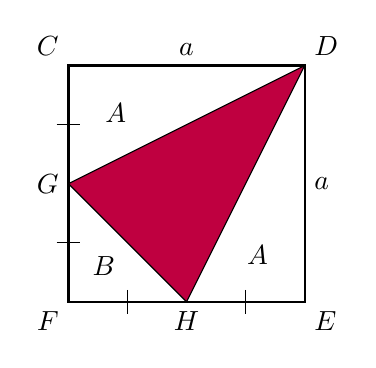
\begin{tikzpicture}[scale=1.5]
		\draw[thick] (-1,1) -- (1,1) -- (1,-1) -- (-1,-1) -- cycle;
		\draw[][fill=purple] (-1,0) -- (0,-1) -- (1,1) -- cycle;
		
		\node[above left] at (-1,1) {$C$};
		\node[above right] at (1,1) {$D$};
		\node[below right] at (1,-1) {$E$};
		\node[below left] at (-1,-1) {$F$};
		\node[left] at (-1,0) {$G$};
		\node[below] at (0,-1) {$H$};
		
		\node[above] at (0,1) {$a$};
		\node[right] at (1,0) {$a$};
		
		\draw (-1.1,0.5) -- (-0.9,0.5);
		\draw (-1.1,-0.5) -- (-0.9,-0.5);
		\draw (-0.5,-0.9) -- (-0.5,-1.1);
		\draw (0.5,-0.9) -- (0.5,-1.1);
		
		\node at (-0.6,0.6) {$A$};
		\node at (0.6,-0.6) {$A$};
		\node at (-0.7,-0.7) {$B$};
		
		\end{tikzpicture}
	\end{center}
	
	% Reasoning
	\paragraph{Reasoning}
	\begin{quotation}
	
	$\triangle DCG$ and $\triangle DEH$ are both right triangles with leg lengths $a$ and $\frac{a}{2}$, which means that they have equal area (denoted as $A$). The triangle area formula is applied to deduce the expression for $A$ (2): $\frac{1}{2}bh \rightarrow A=\frac{1}{2}(a)(\frac{a}{2})=\frac{a^2}{4}$. The area of $\triangle GFH$ is denoted as $B$ and whose expression is deduced likewise: $\frac{1}{2}bh \rightarrow B=\frac{1}{2}(\frac{a}{2})(\frac{a}{2})=\frac{a^2}{8}$. The area for this square, according to the rectangle area formula $bh$, is $a^2$ (1).
	
	Thus, the composed expression for the solution is $a^2-2A-B$ where $A=\frac{a^2}{4}$ and $B=\frac{a^2}{8}$. It is simplified as follows:
	\begin{center}
		\begin{tabular}{l | l}
			$a^2-2(\frac{a^2}{4})-\frac{a^2}{8}$ & Substitute $A$ and $B$ \\
			$a^2-\frac{a^2}{2}-\frac{a^2}{8}$ & Simplify 2nd expression \\
			$a^2-\frac{4a^2}{8}-\frac{a^2}{8}$ & Match denominators for subtraction \\
			$a^2-\frac{5}{8}a^2$ & Combine fractions and extract $a^2$ \\
			$a^2(1-\frac{5}{8})$ & Apply the distributive property \\
			$\frac{3}{8}a^2$ & Simplify \\
		\end{tabular}
	\end{center}
	
	The solution to this problem is therefore $\boxed{\frac{3}{8}a^2}$.
	\end{quotation}
	
	\paragraph{External References}
	
	\begin{enumerate}
		\item Textbook Ch. 9, Pg. 589: Area of Parallelograms
		\item Textbook Ch. 9, Pg. 590: Area of Triangles and Trapezoids
	\end{enumerate}

\end{document}